\section{Android-sovellusten testaamisen perusteet}

Pitäiskö tässä luvussa olla jotain ylipäänsä testaamisen perusteita, vai riittääkö että johdannossa sivutaan aihetta?

\subsection{Testaamisen peruskäsitteitä}

Testitapaus (test case) on yksittäinen testi, jolle on määritelty syötteet, suoritusehdot ja läpäisykriteerit. Testisarja (test suite) taas on joukko testitapauksia. Testisarja voi myös koostua useasta testisarjasta, jolloin esimerkiksi ohjelman jokaiselle komponentille voi olla oma testisarjansa ja yksi testisarja kattaa sitten kaikki yksittäisten komponenttien testisarjat. \cite[153]{testing}

Yksikkötestauksella (unit testing) tarkoitetaan testejä, joiden kohteena on pienimmät mahdolliset ohjelmakomponentit. Olio-ohjelmoinnissa tämä tarkoittaa useimmiten yksittäistä luokkaa, koska yksittäiset metodit vaikuttavat olion tilaan ja siten metodien toimintaan. \cite[282-286]{testing}. JUnit\cite{junit} on Javan standardi yksikkötestaustyökalu.

Yksikkötestaus on useimmiten valkoinen laatikko -testausta (white box testing / structural testing / glass box testing), jolloin testejä voidaan kirjoittaa ohjelmakoodin perusteella. Testeiltä voidaan vaatia esimerkiksi tiettyä koodikattavuutta, jolloin varmistetaan, että mahdollisimman suuri osa ohjelmakoodista tulee suoritettua testien aikana.\cite[154]{testing}

Toiminnallisessa testauksessa (functional testing) testattavan ohjelman sisäistä rakennetta ei tunneta vaan ollaan kiinnostuttu vain syötteistä ja niitä vastaavista tulosteista. Toiminnallista testausta voidaan kutsua myös musta laatikko -testaukseksi (black box testing) (varmista jostain toisesta lähteestä että nämä ovat oikeasti synonyymi, wikipedian mukaan ei ole vaan functional on black boxin alalaji!) Toiminnallisessa testauksessa ollaan kiinnostuttu ohjelman käyttäjälle näkyvästä toiminnasta ja niitä voidaan tehdä esimerkiksi ohjelman määrittelyn pohjalta.\cite[161-162]{testing}

Järjestelmätestauksessa (system testing) testataan koko järjestelmää, se perustuu ohjelman havaittavaan toimintaan ja se on itsenäinen suhteessa ohjelman toteutukseen. Jos ohjelma läpäisee järjestelmätestit, sen voi olettaa olevan vapaa tunnetuista bugeista.\cite[418-421]{testing}

Hyväksyntätestien (acceptance tests) tarkoitus on kertoa, onko ohjelma valmist julkaistavaksi. Hyväksyntätesteissä ei etsitä vikoja ohjelmasta, vaan yritetään varmistaa sen riittävä laatutaso. Hyväksyntätestit ovat usein tilastollisia: niissä mitataan ohjelman luotettavuutta, saavutettavuutta tai häiriötiheyttä. Ongelmana tällaisessa testauksessa on, että vaatii hyvin paljon testiainestoa ennen kuin voidaan olla varmoja ohjelman riittävästä laadusta. Usein hyväksyntätestauksessa käytetään alfa- ja beta-testausta, jolloin ohjelman käyttäjät pääsevät testaamaan ohjelmaa ja raportoimaan sen laadusta.\cite[421-423]{testing}

Mockaus (suomennos?) on tekniikka, joka helpottaa yksikkötestien kirjoittamista. Yksikkötestien ulkoiset riippuvuudet voidaan korvata testeissä kontrolloitavilla mock-olioilla. Tällöin testit ovat vakaampia, koska ulkopuolisten komponenttien muokkaus ei vaikuta testeihin, testin haluttuun lopputulokseen vaikuttava ympäristö on helppo saada haluttuun muotoon. Tällöin testien on helppo testata myös sellaisia olosuhteita, jotka ovat harvinaisia, tai vaikea saada muokattua. Lisäksi mockaamalla voidaan korvata vielä tekemättömät ulkoiset riippuvuudet mock-toteutuksilla. \cite{mocking}

Model based Testing?

\subsection{Mikä on hyvä testityökalu?}

Mm?

\subsection{Android SDK:n mukana tulevia testityökaluja}

\begin{figure}[htb]
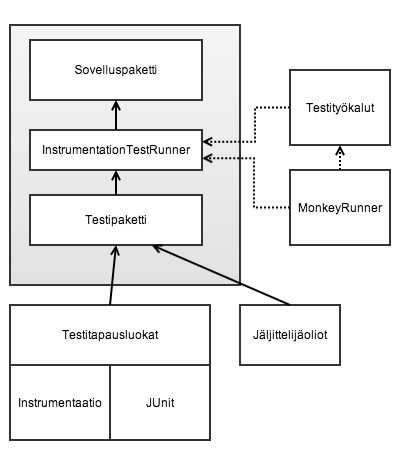
\includegraphics[width=100mm]{test_framework.png}
\caption{placeholder omalle kuvalle} \label{test_framework}
\end{figure}

Androidin SDK:n (suomennos!) mukana tulee monia testaustyökaluja. Testejä voi ajaa joko emulaattorilla tai suoraan puhelimessa.

Androidin testisarjat(suite?) perustuvat JUnit-työkaluun. Puhdasta JUnitia voi käyttää sellaisen koodin testaamiseen, joka ei kutsu Androidin rajapintaa tai sitten voi käyttää Androidin JUnit-laajennusta Android-komponenttien testaukseen. Laajennus tarjoaa komponenttikohtaiset test case (suomennos?) luokat. Nämä luokat tarjoavat apumetodeita mock-olioiden(suomennos?) luomiseen ja komponentin elinkaaren hallintaan. Androidin JUnit-toteutus mahdollistaa JUnitin versio 3:n mukaisen testityylin, ei uudempaa versio 4:n mukaista.\cite{android}

Katso kuva \ref{test_framework}

\subsection{Komponenttikohtaiset testiluokat}

Android tarjoaa aktiviteeteille, palveluille ja sisällöntarjoajille jokaiselle oman testiyläluokkansa, joka mahdollistaa komponenttikohtaisten testien helpomman toteutuksen.

Aktiviteettien testauksessa Androidin JUnit-laajennus on tärkeä, koska aktiviteeteilla on monimutkainen elinkaari, joka perustuu paljolti callback-metodeihin (suomennos), joiden suora kutsuminen ei ole mahdollista. Aktiviteettien testauksen pääyläluokka on InstrumentationTestCase. Sen avulla on mahdollista käynnistää, pysäyttää ja tuhota testattavana oleva aktiviteetti halutuissa kohdissa. Lisäksi sen avulla voi mockata järjestelmäolioita, kuten Contexteja ja Applicationseja. Tämä mahdollistaa testin eristämisen muusta järjestelmästä ja Intentien luomisen testiä varten. Lisäksi yliluokassa on metodit käyttäjäinteraktion, kuten kosketus- ja näppäimistötapahtumien lähettämiseen suoraan testattavalle luokalle.

Aktiviteettien testaamiseen on kaksi olennaista välitöntä yliluokkaa, ActivityUnitTestCase ja ActivityInstrumentationTestCase2. ActivityUnitTestCase on tarkoitettu luokan yksikkötestaamiseen siten, että se on eristetty Android-kirjastoista. Näitä testejä voi ajaa suoraan IDEstä ja tarvittaessa Android-kirjaston mockaamiseen on käytössä MockApplication-olio. ActivityInstrumentationTestCase2 taas on tarkoitettu toiminnalliseen testaukseen tai useamman aktiviteetin testaamiseen. Ne ajetaan normaalissa suoritusympäristössä emulaattorilla tai Android-laitteessa. Aikeiden mockaus on mahdollista, mutta testin eristäminen muusta tuotantojärjestelmästä ei ole mahdollista.

Palveluiden testaaminen on paljon yksinkertaisempaa kuin aktiviteettien. Ne toimivat eristyksessä muusta järjestelmästä, joten testattaessakaan ei tarvita Androidin instrumentaatiota. Android tarjoaa ServiceTestCase-yliluokan palveluiden testaamiseen. Se tarjoaa mock-oliot Application- ja Context-luokille, joten palvelun saa testattua eristettynä muusta järjestelmästä. Testiluokka käynnistää testattavan palvelun vasta kutsuttaessa sen startService() tai bindService()-metodia, jolloin mock-oliot voi alustaa ennen palvelun käynnistymistä. Mock-olioiden käyttö palveluiden testaamisessa paljastaa myös mahdolliset huomaamatta jääneet riippuvuudet muuhun järjestelmään, koska mock-oliot heittävät poikkeuksen, mikäli niihin tulee metodikutsu, johon ei ole varauduttu.

Sisällöntarjoajien testaaminen on erityisen tärkeää, jos sovellus tarjoaa sisällöntarjoajiaan muiden sovellusten käyttöön. Tällöin on myös olennaista testata niitä käyttäen samaa julkista rajapintaa, jota muut sovellukset joutuvat käyttämään kommunikoidessaan sisällöntarjoajien kanssa. Sisällöntarjoajien testauksen yliluokka on ProviderTestCase2, joka tarjoaa käyttöön mock-oliot ContentResolveriosta ja Contextista, jolloin sisällöntarjoajia voi testaja eristyksissä muusta sovelluksesta. Yliluokka tarjoaa myös metodit sovelluksen oikeuksien testaamisen. Contextin mock-olio mahdollistaa tiedosto- ja tietokantaoperaatiot, mutta muut Androidin kirjastokutsut on toteutettu stubeina. Lisäksi tiedon kirjoitusosoite on uniikki testissä, joten testien ajaminen ei yliaja varsinaista sovelluksen tallentamaa tietoa. Sisällöntarjoajatestit ajetaan emulaattorissa tai Android-laitteella. \cite{android}

\subsection{Monkeyrunner}

Monkeyrunner tarjoaa rajapinnan, jolla android-sovellusta voi ohjata laitteessa tai emulaattorissa. Se on lähinnä tarkoitettu toiminnallisten testien (functional tests, onko oikea suomennos?) sekä yksikkötestien ajamiseen, mutta soveltuu myös muihin tarkoituksiin. Sen avulla voi esimerkiksi asentaa sovelluksia, ajaa testisarjoja ja sovelluksia ja lähettää niihin syötteitä. Lisäksi monkeyrunnerilla voi ottaa eri kohdista kuvakaappauksia ja verrata niitä referenssikuviin. Tällä tavalla voidaan tehdä esimerkiksi regressiotestausta.

Monkeyrunnerilla voidaan testata yhtä aikaa esimerkiksi monia eri emulaattoreita tai useita laitteita, jolloin voidaan tehdä fragmentaatiotestausta. Monkeyrunner on myös laajennettavissa, jolloin sitä voi käyttää muihinkin tarkoituksiin. Monkeyrunneria ohjataan pythonilla ja se on toteutettu jythonilla, joka on javan virtuaalikoneessa pyörivä python-toteutus.\cite{android}

\subsection{Monkey}

Monkey on Androidin mukana tuleva työkalu, jota voi ajaa emulaattorissa tai Android-laitteessa ja joka tuottaa pseudosatunnaisia syötteitä ohjelmalle, kuten painalluksia, eleitä sekä järjestelmätason viestejä. Monkeytä voi käyttää esimerkiksi sovelluksen stressitestaukseen tai fuzz-testaukseen.

Monkeylle voi antaa jonkin verran sen toimintaa ohjaavia parametreja. Ensinnäkin testisyötteiden määrää ja tiheyttä voi rajoittaa. Toiseksi erityyppisten syötteiden osuutta voi säätää. Kolmanneksi testauksen voi rajoittaa tiettyyn pakettiin sovelluksessa. Tällöin Monkey pysäyttää testauksen, jos se on ajautuu muihin kuin haluttuun osaan sovelluksesta. Neljänneksi Monkeyn tulosteiden määrää ja tarkkuutta voi säätää.

Monkey pystäyttää testin, jos ohjelmasta lentää käsittelemätön poikkeus tai jos järjestelmä lähettää sovellus ei vastaa -virheviestin. Näissä tapauksissa Monkey antaa raportin virheestä ja miten se syntyi. Monkey voi myös haluttaessa tehdä profilointiraportin testistä.\cite{android}

\subsection{Androidin testaustyökalujen arviointia}

Mikä on hyvällä mallilla, mihin tarvitaan lisätyökaluja